% !TEX spellcheck = nl_NL
\chapter{Inleiding}
Bij het informatica-vak Functioneel Programmeren, gegeven aan de Universiteit Twente, gebruiken studenten Haskell om fundamentele concepten van functioneel programmeren te bestuderen. Hierbij wordt door de studenten veel gebruik gemaakt van grafische weergaven om de werking van hun code inzichtelijk te maken. Het gebruik van Haskell voor het maken van grafische weergaven blijkt vaak redelijk gecompliceerd en limiteert studenten doordat zij zich bezig moeten houden met minder intuïtieve en minder essentiële aspecten van Haskell.

Om de focus binnen Functioneel Programmeren op de essentie te houden, was al een grafische omgeving ontwikkeld op basis van de Gloss grafische library. De interface tussen de code van de student en de grafische interface is eenvoudig en bruikbaar, het bevat echter een aantal nadelen. Het werkt niet goed op ieder platform, mist een aantal functionaliteiten en de prestatie is niet uitstekend. Vanuit de tekortkomingen van dit oude systeem zijn requirements geformuleerd voor een nieuwe omgeving die de oude op termijn zou moeten vervangen. In \autoref{hoofdstuk:requirements} wordt uitgebreid ingegaan op de requirements voor deze nieuwe omgeving.

In dit project is als antwoord op bovenstaande vraag \emph{Canvas.hs} ontwikkeld; een omgeving die Haskell-gebruikers in staat stelt op eenvoudige wijze grafische elementen op een HTML5 canvas te presenteren. Figuur \ref{fig:overzicht_canvas.hs} geeft een overzicht van de verschillende onderdelen van Canvas.hs.

\begin{figure}
\begin{center}
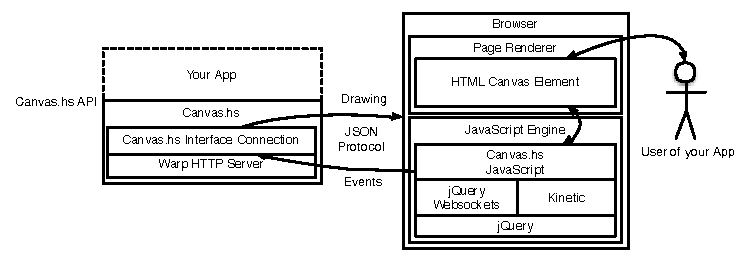
\includegraphics[keepaspectratio,width=\textwidth]{./images/architectuur_overzicht.pdf}
\caption{Overzicht  van Canvas.hs}
\label{fig:overzicht_canvas.hs}
\end{center}
\end{figure}

\subsubsection{Canvas.hs}
Canvas.hs is ontwikkeld met het oog op gebruiksgemak en eenvoud zonder de mogelijkheid tot uitbreiding en het toevoegen van geavanceerde functionaliteit onnodig te beperken.

Canvas.hs is als library te installeren via \emph{Cabal}, de package manager voor Haskell programma's. In \fullref{sec:gebruikershandleiding} kan gelezen worden hoe de library gebruikt kan worden. Als een Haskell programma via de aangeboden API de library aanroept, zal een zeer lichte HTTP en Websocket server opgestart worden. De library zal vervolgens een browser opstarten. Deze browser laadt de JavaScript code van de library en toont vervolgens een HTML5 canvas waar op getekend kan worden door het Haskell programma van de gebruiker. In \autoref{hoofdstuk:ontwerp} wordt het ontwerp van Canvas.hs uitgebreider beschreven.

De ontwikkelde library is uitgebreid getest. Dit geldt zowel voor de geschreven Haskell code als de JavaScript code. In \autoref{hoofdstuk:testplan} staat het testplan dat bij het maken van tests gebruikt is en in \autoref{hoofdstuk:resultaten} staan de resultaten van de tests.

\subsubsection{Organisatie}
Bij de ontwikkeling van Canvas.hs is vooraf een managementmethode vastgesteld. Daarnaast is er tooling gebruikt om de samenwerking tussen ontwikkelaars te vergemakkelijken. \autoref{hoofdstuk:organisatie} beschrijft hoe dit alles is ingericht en \autoref{hoofdstuk:evaluatie} beschrijft hoe de afspraken en tools uiteindelijk zijn toegepast en wat de ervaringen hiermee waren.

\subsubsection{Uitbreidingen}
In \autoref{hoofdstuk:evaluatie} worden enkele knelpunten binnen het ontwikkelde Canvas.hs besproken en in \autoref{hoofdstuk:conclusie} worden aanbevelingen gedaan over hoe deze knelpunten verholpen kunnen worden in toekomstige versies. Verder is Canvas.hs opgezet zodat deze gemakkelijk is uit te breiden. In \fullref{sec:uitbreiden} is te lezen hoe Canvas.hs uitgebreid kan worden met nieuwe shapes of events.


